\documentclass[tikz,border=4pt]{standalone}
% Paleta y fuentes compartidas por el libro y las figuras (única fuente de verdad).
\RequirePackage{xcolor}
\definecolor{oxido}{HTML}{B7410E}
\definecolor{cobre}{HTML}{D27D2D}
\definecolor{carbon}{HTML}{2B2B2B}
\definecolor{azul}{HTML}{1F5F8B}
\definecolor{arena}{HTML}{F4EDE4}

\usepackage{fontspec}
\setsansfont{FiraSans}[Extension=.otf,UprightFont=*-Regular,BoldFont=*-SemiBold,ItalicFont=*-Italic,BoldItalicFont=*-SemiBoldItalic]
\setmonofont{FiraMono}[Extension=.otf,UprightFont=*-Regular,BoldFont=*-Medium,Scale=0.95]
\usetikzlibrary{positioning,arrows.meta,calc,decorations.pathreplacing}
\begin{document}
\sffamily\small
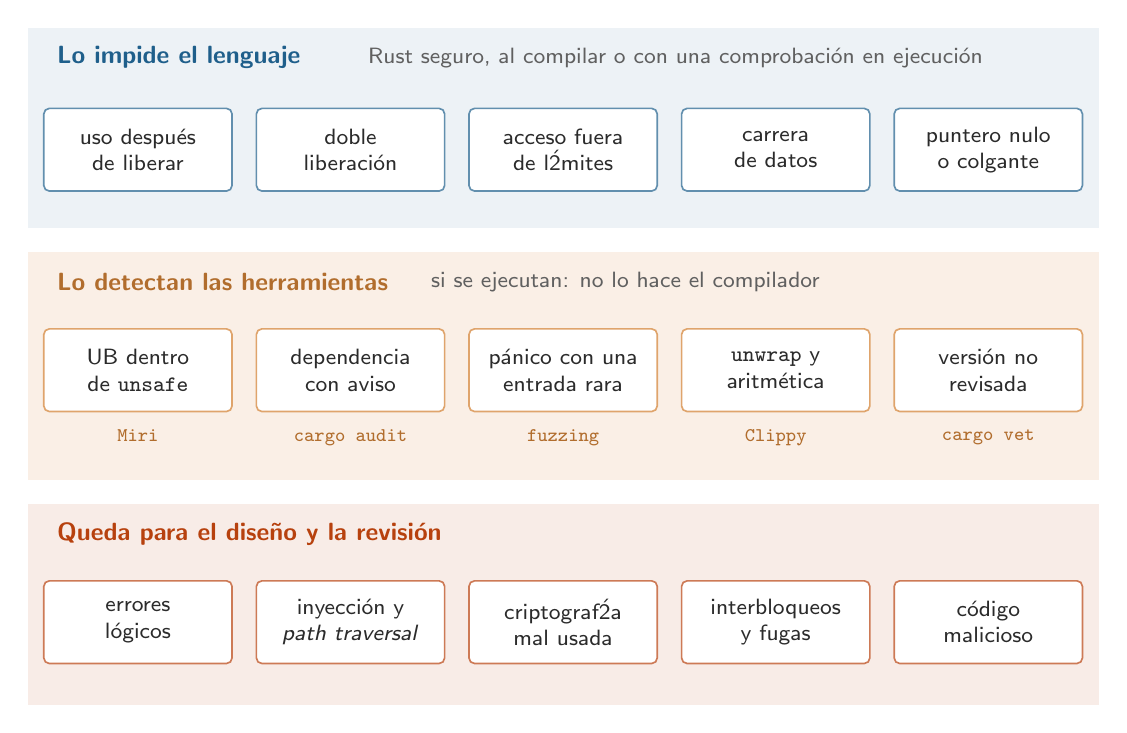
\begin{tikzpicture}[
  titulo/.style={font=\sffamily\small\bfseries,anchor=west},
  sub/.style={font=\sffamily\footnotesize,text=carbon!75,anchor=west},
  ficha/.style={draw=#1!70,fill=white,rounded corners=2pt,line width=0.6pt,
    font=\sffamily\footnotesize,text=carbon,align=center,
    text width=2.25cm,minimum height=1.05cm,inner sep=2pt,
    execute at begin node={\hyphenpenalty=10000}},
  herr/.style={font=\ttfamily\scriptsize,text=#1}]
  % ---- Capa 1: el lenguaje ----
  \fill[azul!8] (0,0) rectangle (13.6,-2.55);
  \node[titulo,text=azul] at (0.25,-0.38) {Lo impide el lenguaje};
  \node[sub] at (4.2,-0.38) {Rust seguro, al compilar o con una comprobación en ejecución};
  \foreach \t [count=\i from 0] in {uso después\\de liberar,doble\\liberación,
      acceso fuera\\de límites,carrera\\de datos,puntero nulo\\o colgante}
    {\node[ficha=azul] at (1.4+\i*2.7,-1.55) {\t};}
  % ---- Capa 2: herramientas ----
  \fill[cobre!12] (0,-2.85) rectangle (13.6,-5.75);
  \node[titulo,text=cobre!80!carbon] at (0.25,-3.23) {Lo detectan las herramientas};
  \node[sub] at (5.0,-3.23) {si se ejecutan: no lo hace el compilador};
  \foreach \t/\h [count=\i from 0] in {UB dentro\\de \texttt{unsafe}/Miri,
      dependencia\\con aviso/cargo audit,
      pánico con una\\entrada rara/fuzzing,
      \texttt{unwrap} y\\aritmética/Clippy,
      versión no\\revisada/cargo vet}
    {\node[ficha=cobre] (h\i) at (1.4+\i*2.7,-4.35) {\t};
     \node[herr=cobre!80!carbon,below=1mm of h\i] {\h};}
  % ---- Capa 3: diseño y revisión ----
  \fill[oxido!10] (0,-6.05) rectangle (13.6,-8.6);
  \node[titulo,text=oxido] at (0.25,-6.43) {Queda para el diseño y la revisión};
  \foreach \t [count=\i from 0] in {errores\\lógicos,inyección y\\\emph{path traversal},
      criptografía\\mal usada,interbloqueos\\y fugas,código\\malicioso}
    {\node[ficha=oxido] at (1.4+\i*2.7,-7.55) {\t};}
\end{tikzpicture}
\end{document}
